% rv-123.tex
% definition-epistemologie-enaction.tex

%-------------------------------------------------------------------------
%\documentclass[aspectratio=169]{beamer}
\documentclass{beamer}
%-------------------------------------------------------------------------

%-------------------------------------------------------------------------
\mode<presentation>
{
\usetheme{PoS}
}
%-------------------------------------------------------------------------

%-------------------------------------------------------------------------
\title[Réalité virtuelle]{}
\author[jacques.tisseau@enib.fr]{}
\date[Pint of Science --- Brest, 16/05/2018]{}
\institute[]{}
%-------------------------------------------------------------------------

\graphicspath{{./fig/}}
\arrayrulecolor{orange}

\newmdenv[linecolor=orange!40,backgroundcolor=orange!40,roundcorner=10pt]{infobox}

%-------------------------------------------------------------------------
\begin{document}
%-------------------------------------------------------------------------

%------------------------------------------
\begin{frame}
%------------------------------------------
\vspace*{3mm}

\includegraphics[height=1.225cm]{logo-cerv}\hfill
\includegraphics[height=1.225cm]{logo-pintofscience}\includegraphics[height=1.225cm]{logo-pintofscience}\includegraphics[height=1.225cm]{logo-pintofscience}

\setbeamercolor{block body}{fg=white,bg=orange}
\begin{block}{}
\centerline{\huge\bf
\begin{tabular}{c}
\mbox{}\\
\cellcolor{orange}\color{white}Réalité virtuelle\\
\mbox{}
\end{tabular}
}
\end{block}
\setbeamercolor{block body}{fg=black,bg=white}
\null\vfill

\centerline{\LARGE Jacques Tisseau}
\null\vfill

\noindent
%\mbox{}\hfill
\begin{minipage}{1.5cm}
\includegraphics[height=1.3cm]{logo-cnrs}
\end{minipage}
\hspace{-4mm}
\begin{minipage}{3cm}
\includegraphics[height=1.3cm]{logo-labsticc}
\end{minipage}
\hfill
\begin{minipage}{2.75cm}
\begin{center}
%\includegraphics[height=1.75cm]{logo-pintofscience}\\
%16/05/2018
\end{center}
\end{minipage}
\hfill
\begin{minipage}{2.75cm}
\includegraphics[height=1.75cm]{logo-enib}
\end{minipage}
%\hfill
\mbox{}

\end{frame}
\note{
Bonjour.

Depuis une petite trentaine d'années que je travaille dans le domaine de la réalité virtuelle,
on m'a souvent demandé : « mais en deux mots simplement, c'est quoi la réalité virtuelle ? »
En deux mots, il est difficile de faire plus concis que « réalité » « virtuelle ».
Mais si on pose la question, c'est que cette expression pose problème.

CLIC
}
%------------------------------------------

%------------------------------------------
\begin{frame}
\frametitle{Plan}
%------------------------------------------
\LARGE
\mbox{}\hfill\begin{minipage}{11cm}\bf
\begin{enumerate}
\item La réalité virtuelle en deux mots
\vspace*{1cm}

\item L'expérimentation in virtuo
\vspace*{1cm}

\item L'énaction en action
\end{enumerate}
\end{minipage}
\hfill\mbox{}

\end{frame}
\note{}
%------------------------------------------


%------------------------------------------
\begin{frame}
\frametitle{Les mots pour le dire}
%------------------------------------------

%\begin{columns}[T]
%\column{4cm}
%%\noindent\framebox[4cm]{$\rule{0mm}{6.5cm}$}
%\column{10cm}
%\noindent
\begin{center}
\begin{tikzpicture}
\draw (0,0) node {
	\begin{minipage}{10cm}
	\begin{minipage}{2.2cm}\includegraphics[width=2cm]{artaud-livre-1.jpg}\end{minipage}
	\begin{minipage}{7.7cm}
		\textbf{Antonin ARTAUD} ( \includegraphics[width=0.5cm]{france.png}\ 1932)\\
		\mbox{}\\
		« la réalité virtuelle du théâtre »\\[2mm]
		\begin{minipage}{7.5cm}\tiny  
		Le théâtre alchimique (1932),\\
		{\em dans} Le théâtre et son double, Paris, 1938
		\end{minipage}
	\end{minipage}
	\end{minipage}
};
\end{tikzpicture}

	\pause

%\noindent
\begin{tikzpicture}
\draw (0,0) node {
	\begin{minipage}{10cm}
	\begin{minipage}{2.2cm}\includegraphics[width=2cm]{lanier-1.jpg}\end{minipage}
	\begin{minipage}{7.7cm}
		\textbf{Jaron LANIER} ( \includegraphics[width=0.5cm]{usa.png}\ 1989)\\
		\begin{minipage}{7.5cm}\small« virtual reality », « alternate reality »,\\« expansion of reality », « artificial reality »\end{minipage}\\[2mm]
		\begin{minipage}{7.5cm}\tiny  
		\tiny An interview with Jaron Lanier, Whole Earth Review, Fall 1989
		\end{minipage}
	\end{minipage}
	\end{minipage}
};
\end{tikzpicture}
\end{center}
	
%\end{columns}


\end{frame}
\note{
Alors d'où vient cette expression ?

Il semblerait qu'on la trouve pour la première fois en 1932 dans un texte d'Antonin Artaud,
homme de théâtre français du début du 20ème siècle. 
Antonin Artaud voit dans le théâtre un entre deux, un monde entre réel et imaginaire, 
qui dans l'interaction de toutes ses modalités (le texte, la mise en scène, le jeu des acteurs, 
le décor, les lumières, les sons...) provoque une sorte d'alchimie qui non seulement révèle le
monde tel qu'il est mais participe à sa transformation en lui donnant un nouveau sens.

CLIC

Mais c'est avec Jaron Lanier, informaticien et artiste américain contemporain, que l'expression
entre dans la sphère scientifique et technique.
Technique d'abord, car c'est à l'occasion d'un salon professionnel, que la société VPL Research
cofondée par Jaron Lanier, dévoile ses premières interfaces de réalité virtuelle avec en vedette
un gant de données qui permettait d'immerger sa propre main dans un modèle numérique.
Lors d'une interview à la revue « The Whole Earth Review », il développe l'idée d'une
réalité virtuelle comme une « réalité alternative », une « extension de la réalité » ou encore une 
« réalité artificielle ».

Mais l'expression réalité réalité virtuelle n'en demeure pas moins une figure de style 
plus littéraire que scientifique.

CLIC
}
%------------------------------------------

%------------------------------------------
\begin{frame}
\frametitle{Entre deux}
%------------------------------------------
%\begin{columns}[T]
%\column{4cm}
%%\noindent\framebox[4cm]{$\rule{0mm}{6.5cm}$}
%\column{10cm}
\begin{columns}[T]
	\column{5cm}
	\onslide<2->{\textbf{Oxymore}\\[2mm]

	{\tiny « clair obscur », « aigre doux »,\\ « mort vivant », « silence éloquent »
	\\\ldots\\[-1mm]
	« réalité virtuelle »}
	}
	
	
	\vspace*{1mm}
	
	\begin{itemize}
	\item<1-> \alert{\bf usage courant :}
	
		le virtuel s'oppose au réel
	\end{itemize}
	
	\column{5cm}
	\onslide<4->{\textbf{Pléonasme}\\[2mm]
	
	{\tiny « monter en haut », « au jour d'aujourd'hui »,\\ « prévoir à l'avance~», « collaborer ensemble~»\\\ldots\\[-1mm]
	« réalité virtuelle »}
	}
	\vspace*{1mm}
	
	\begin{itemize}
	\item<3-> \alert{\bf constructivisme :}
	
	la réalité comme représentation du réel,
	construction de l'esprit
	\end{itemize}
\end{columns}
\vspace*{4mm}

\onslide<5->{
\centerline{
\begin{tabular}{|lcr|}
\hline
\makebox[1.8cm][l]{latent} & \multirow{3}{*}{\includegraphics[width=1.75cm]{levy-livre.jpg}} & \makebox[1.8cm][r]{manifeste}\\
\hline
& & \\
possible & & réel \\
 & & \\
virtuel & & actuel\\[2.7mm]
\hline
\end{tabular}
}}
%\end{columns}

\end{frame}
\note{
En effet, du point de vue du grand public,
le virtuel s'oppose au réel.
Le réel, c'est la chose qui existe, qui résiste et qui subsiste.
Ce qui ne serait pas le cas du virtuel.

CLIC

Il s'agit donc d'une figure de style
appelée « oxymore », expression composée de termes qui s'opposent l'un l'autre.
Comme le « clair obscur » des peintres, l'« aigre doux » des cuisiniers, le « mort vivant »
de la science-fiction ou encore le « silence éloquent » des interlocuteurs.
Autant d'expressions qui se situent entre deux extrêmes pour créer une réalité « poétique »
surprenante.
La réalité virtuelle serait donc un oxymore de plus !

CLIC

Mais, si l'on se fie aux épistémologies plus récentes, comme le constructivisme,
la réalité ne serait pas le réel mais plutôt une représentation du réel : une construction 
de l'esprit et relèverait donc plus du virtuel que du réel.
On aurait donc affaire à un autre type de figure de style : le pléonasme.

CLIC

Comme « monter en haut », « au jour d'aujourd'hui », « prévoir à l'avance » ou « collaborer ensemble »,
autant d'expressions qui tendent à renforcer l'idée principale.
La réalité virtuelle serait donc un pléonasme de plus !

CLIC

Nous n'allons pas nous perdre ici dans cet entre deux, entre oxymore et pléonasme,
et pour y voir plus clair sur la relation du réel au virtuel, je vous conseille la lecture
du petit livre de Pierre Lévy qui précise la place du virtuel par rapport au réel, à l'actuel et au possible.

CLIC
}
%------------------------------------------

%------------------------------------------
\begin{frame}
\frametitle{Une définition consensuelle}
%------------------------------------------
%\begin{columns}[T]
%\column{4cm}
%%\noindent\framebox[4cm]{$\rule{0mm}{6.5cm}$}
%\column{10cm}
\begin{minipage}{11cm}\color<2->{lightgray}
La réalité virtuelle est un domaine scientifique et technologique
exploitant l'informatique et des interfaces comportementales
%\pause
en vue de \alert<2->{\textbf<2->{simuler}} dans un monde virtuel 
\alert<2->{\textbf<2->{le comportement d'entités}} 3D,
%\pause
qui sont \alert<2->{\textbf<2->{en interaction en temps réel entre elles}}
%\pause
et \alert<2->{\textbf<2->{avec un ou des utilisateurs}}
en immersion pseudo-naturelle par l'intermédiaire de canaux sensori-moteurs.
\vspace*{2mm}

%\pause
\mbox{}\hfill \href{http://caor.mines-paristech.fr/caor/interlivre}{\alert{\bf « Le traité de la réalité virtuelle »}}\\
\mbox{}\hfill \footnotesize Presses de l'Ecole des Mines de Paris (2003-2009)
\end{minipage}
\vspace*{3mm}
 
\begin{minipage}{1.5cm}
\includegraphics[width=1.25cm]{trv1.jpg}\\
\tiny Tome 1
\end{minipage}
\hfill
\begin{minipage}{1.5cm}
\includegraphics[width=1.25cm]{trv2.jpg}\\
\tiny Tome 2
\end{minipage}
\hfill
\begin{minipage}{1.5cm}
\includegraphics[width=1.25cm]{trv3.jpg}\\
\tiny Tome 3
\end{minipage}
\hfill
\begin{minipage}{1.5cm}
\includegraphics[width=1.25cm]{trv4.jpg}\\
\tiny Tome 4
\end{minipage}
\hfill
\begin{minipage}{1.5cm}
\includegraphics[width=1.25cm]{trv5.jpg}\\
\tiny Tome 5
\end{minipage}
%\end{columns}

\end{frame}
\note{
Mais, c'est à la communauté scientifique de préciser les termes qu'elle emploie.
Et c'est ce qu'a fait la communauté française au début des années 2000,
lors de l'élaboration collective d'un traité de la réalité virtuelle, 
en proposant cette définition technique et consensuelle de la réalité virtuelle.

Ce traité de plus de 2000 pages structurées en 5 tomes, propose donc une définition 
qui ne tient évidemment pas en deux mots.
Et pour y voir plus clair, retenons ici
que « la réalité virtuelle est une simulation du comportement d'entités en interaction 
en temps réel entre elles et avec un ou des utilisateurs. »

CLIC
}
%------------------------------------------

%------------------------------------------
\begin{frame}<presentation>
\frametitle{Immersion, interaction, autonomie}
%------------------------------------------
%\centerline{\multiinclude[format=pdf,graphics={width=0.9\textwidth}]{rv}}
$$\begin{tikzpicture}[scale=2.4]
\draw (0,0) -- (1,0);
\draw[thick,->] (1,0) -- (1.25,0);
\fill[color=bleu] (1,0) circle(0.125/2);
\draw (1.25,0) node[right]{\textbf{interaction}};
\draw (0,0) -- ({-2/(3*sqrt(3))},-2/3);
\draw[thick,->] ({-2/(3*sqrt(3))},-2/3) -- ({-1/sqrt(3)},-1);
\fill[color=bleu] ({-2/(3*sqrt(3))},-2/3) circle(0.125/2);
\draw ({-1/sqrt(3)},-1) node[below]{\textbf{immersion}};
\draw[fill=bleu,opacity=0.2] ({-2/(3*sqrt(3))},-2/3) -- ({1 - 2/(3*sqrt(3))},-2/3) -- (1,0) -- (0,0) -- cycle;
\draw ({(1 - 2/(3*sqrt(3)))/2},-1/3) node[rotate=26]{\textbf{\color{bleu}présence}};
\fill[color=bleu] ({1 - 2/(3*sqrt(3))},-2/3) circle(0.125/2);
\pause
\draw ({-2/(3*sqrt(3)) - 0.03},-2/3) node[left]{\alert{\textbf{\scriptsize cinéma 3D}}};
\draw (1,0) node[above]{\alert{\textbf{\scriptsize jeu vidéo}}};
%\draw (1,0.175) node[above]{\alert{\textbf{\scriptsize jeu}}};
\draw ({1 - 2/(3*sqrt(3))},{-2/3 -0.03}) node[below]{\alert{\textbf{\scriptsize simulateur de transport}}};
%\draw ({1 - 2/(3*sqrt(3))},-2/3-0.14) node[below]{\alert{\textbf{\scriptsize de transport}}};
\pause
\draw (0,0) -- (0,1);
\draw[thick,->] (0,1) -- (0,1.25);
\fill[color=bleu] (0,1) circle(0.125/2);
\draw (0,1.25) node[above]{\textbf{autonomie}};
\draw[dashed] ({-2/(3*sqrt(3))},-2/3) -- ({-2/(3*sqrt(3))},1/3);
\draw[dashed] ({-2/(3*sqrt(3))},1/3) -- (0,1);
\fill[color=bleu] ({-2/(3*sqrt(3))},1/3) circle(0.125/2);
\draw[dashed] (0,1) -- (1,1);
\draw[dashed] (1,1) -- (1,0);
\fill[color=bleu] (1,1) circle(0.125/2);
\draw[dashed] ({-2/(3*sqrt(3))},1/3) -- ({1 - 2/(3*sqrt(3))},1/3);
\draw[dashed] ({1 - 2/(3*sqrt(3))},1/3) -- (1,1);
\draw[dashed] ({1 - 2/(3*sqrt(3))},1/3) -- ({1 - 2/(3*sqrt(3))},-2/3);
\fill[color=bleu,opacity=0.2] ({-2/(3*sqrt(3))},1/3) -- ({1 - 2/(3*sqrt(3))},1/3) -- (1,1) -- (0,1) -- cycle;
\fill[color=bleu,opacity=0.2] ({-2/(3*sqrt(3))},-2/3) -- ({1 - 2/(3*sqrt(3))},-2/3) -- ({1 - 2/(3*sqrt(3))},1/3) -- ({-2/(3*sqrt(3))},1/3) -- cycle;
\fill[color=bleu,opacity=0.2] ({1 - 2/(3*sqrt(3))},-2/3) -- (1,0) -- (1,1) -- ({1 - 2/(3*sqrt(3))},1/3) -- cycle;
\pause
\draw ({0-0.03},1) node[left]{\alert{\textbf{\scriptsize virus}}};
\draw ({-2/(3*sqrt(3)) - 0.03},1/3) node[left]{\alert{\textbf{\scriptsize théâtre virtuel}}};
\draw (1,{1+0.03}) node[above]{\alert{\textbf{\scriptsize fiction interactive}}};
%\draw (1,1+0.175) node[above]{\alert{\textbf{\scriptsize fiction}}};
\pause
\draw ({(1 - 2/(3*sqrt(3)))/2},2/3) node[rotate=26]{\textbf{\color{bleu}in virtuo}};
\draw ({1 - 2/(3*sqrt(3))},1/3+0.2) node{\color{rose}\textbf{\Large RV}};
\fill[color=rose] ({1 - 2/(3*sqrt(3))},1/3) circle(0.2/2);
\end{tikzpicture}$$

\end{frame}
\note{}
%------------------------------------------


%------------------------------------------
\begin{frame}<presentation>
\frametitle{Métaphore de Pinocchio}
%\framesubtitle{Immersion, interaction, autonomie}
%------------------------------------------
%\begin{columns}[T]
%\column{4cm}
%%\noindent\framebox[4cm]{$\rule{0mm}{6.5cm}$}
%\column{10cm}
\begin{tikzpicture}

\begin{scope}
\draw (0,0) -- (1,0);
\draw[thick,->] (1,0) -- (1.25,0);
\fill[color=bleu] (1,0) circle(0.125/2);
\draw (1.25,0) node[right]{\textbf{\tiny interaction}};
\draw (0,0) -- ({-2/(3*sqrt(3))},-2/3);
\draw[thick,->] ({-2/(3*sqrt(3))},-2/3) -- ({-1/sqrt(3)},-1);
\fill[color=bleu] ({-2/(3*sqrt(3))},-2/3) circle(0.125/2);
\draw ({-1/sqrt(3)},-1) node[below]{\textbf{\tiny immersion}};
\draw[fill=bleu,opacity=0.2] ({-2/(3*sqrt(3))},-2/3) -- ({1 - 2/(3*sqrt(3))},-2/3) -- (1,0) -- (0,0) -- cycle;
%\draw ({(1 - 2/(3*sqrt(3)))/2},-1/3) node[rotate=26]{\textbf{\color{bleu}présence}};
\fill[color=bleu] ({1 - 2/(3*sqrt(3))},-2/3) circle(0.125/2);
%\pause
%\draw ({-2/(3*sqrt(3)) - 0.03},-2/3) node[left]{\alert{\textbf{\scriptsize cinéma 3D}}};
%\draw (1,0) node[above]{\alert{\textbf{\scriptsize jeu vidéo}}};
%\draw (1,0.175) node[above]{\alert{\textbf{\scriptsize jeu}}};
%\draw ({1 - 2/(3*sqrt(3))},{-2/3 -0.03}) node[below]{\alert{\textbf{\scriptsize simulateur de transport}}};
%\draw ({1 - 2/(3*sqrt(3))},-2/3-0.14) node[below]{\alert{\textbf{\scriptsize de transport}}};
%\pause
\draw (0,0) -- (0,1);
\draw[thick,->] (0,1) -- (0,1.25);
\fill[color=bleu] (0,1) circle(0.125/2);
\draw (0,1.25) node[above]{\textbf{\tiny autonomie}};
\draw[dashed] ({-2/(3*sqrt(3))},-2/3) -- ({-2/(3*sqrt(3))},1/3);
\draw[dashed] ({-2/(3*sqrt(3))},1/3) -- (0,1);
\fill[color=bleu] ({-2/(3*sqrt(3))},1/3) circle(0.125/2);
\draw[dashed] (0,1) -- (1,1);
\draw[dashed] (1,1) -- (1,0);
\fill[color=bleu] (1,1) circle(0.125/2);
\draw[dashed] ({-2/(3*sqrt(3))},1/3) -- ({1 - 2/(3*sqrt(3))},1/3);
\draw[dashed] ({1 - 2/(3*sqrt(3))},1/3) -- (1,1);
\draw[dashed] ({1 - 2/(3*sqrt(3))},1/3) -- ({1 - 2/(3*sqrt(3))},-2/3);
\fill[color=bleu,opacity=0.2] ({-2/(3*sqrt(3))},1/3) -- ({1 - 2/(3*sqrt(3))},1/3) -- (1,1) -- (0,1) -- cycle;
\fill[color=bleu,opacity=0.2] ({-2/(3*sqrt(3))},-2/3) -- ({1 - 2/(3*sqrt(3))},-2/3) -- ({1 - 2/(3*sqrt(3))},1/3) -- ({-2/(3*sqrt(3))},1/3) -- cycle;
\fill[color=bleu,opacity=0.2] ({1 - 2/(3*sqrt(3))},-2/3) -- (1,0) -- (1,1) -- ({1 - 2/(3*sqrt(3))},1/3) -- cycle;
%\pause
%\draw ({0-0.03},1) node[left]{\alert{\textbf{\scriptsize virus}}};
%\draw ({-2/(3*sqrt(3)) - 0.03},1/3) node[left]{\alert{\textbf{\scriptsize théâtre virtuel}}};
%\draw (1,{1+0.03}) node[above]{\alert{\textbf{\scriptsize fiction interactive}}};
%\draw (1,1+0.175) node[above]{\alert{\textbf{\scriptsize fiction}}};
%\pause
%\draw ({(1 - 2/(3*sqrt(3)))/2},2/3) node[rotate=26]{\textbf{\color{bleu}in virtuo}};
\draw ({1 - 2/(3*sqrt(3))},1/3+0.2) node{\color{rose}\textbf{\tiny RV}};
\fill[color=rose] ({1 - 2/(3*sqrt(3))},1/3) circle(0.2/2);
\end{scope}

\pause

\begin{scope}[xshift=1cm,yshift=-3.6cm]
\draw (0,0) node {\begin{minipage}{2.6cm}
\mbox{}\hfill\textbf{immersion}\mbox{}\\
\centerline{\includegraphics[width=3cm]{pinocchio-immersion.jpg}}
\end{minipage}};
\end{scope}

\pause

\begin{scope}[xshift=4.5cm,yshift=-1.8cm]
\draw (0,0) node {\begin{minipage}{2.6cm}
\mbox{}\hfill\textbf{interaction}\mbox{}\\
\centerline{\includegraphics[width=3cm]{pinocchio-interaction.jpg}}
\end{minipage}};
\end{scope}

\pause

\begin{scope}[xshift=8cm]
\draw (0,0) node {\begin{minipage}{2.6cm}
\mbox{}\hfill\textbf{autonomie}\mbox{}\\
\centerline{\includegraphics[width=3cm]{pinocchio-autonomie.jpg}}
\end{minipage}};
\end{scope}

\end{tikzpicture}

%\end{columns}


\end{frame}
\note{}
%------------------------------------------

%------------------------------------------
\begin{frame}<presentation>
\frametitle{Caverne de Platon revisitée}
%------------------------------------------
%\begin{columns}[T]
%\column{4cm}
%%\noindent\framebox[4cm]{$\rule{0mm}{6.5cm}$}
%\column{10cm}
\alert{\textbf{Réalité Virtuelle :}} vivre une expérience cognitive et sensorimotrice
dans un univers virtuel peuplé d'entités autonomes.
\vspace*{2mm}

\mbox{}\hfill$\rightarrow$ \alert{\bf vivre une expérience de pensée}\mbox{}
\vspace*{5mm}

\pause

\begin{tikzpicture}
\begin{scope}
\draw(0,0) node {\includegraphics[width=5cm]{immersia-1.png}};
\end{scope}

\begin{scope}[xshift=4.5cm,yshift=1cm]
\draw(0,0) node {\includegraphics[width=2.5cm]{rv-periph-1.jpg}};
\end{scope}

\begin{scope}[xshift=7.5cm,yshift=1cm]
\draw(0,0) node {\includegraphics[width=2.5cm]{rv-periph-2.jpg}};
\end{scope}

\begin{scope}[xshift=7.5cm,yshift=-1cm]
\draw(0,0) node {\includegraphics[width=2.5cm]{rv-periph-3.jpg}};
\end{scope}

\begin{scope}[xshift=4.5cm,yshift=-1cm]
\draw(0,0) node {\includegraphics[width=2.5cm]{rv-periph-4.jpg}};
\end{scope}
\end{tikzpicture}
%\end{columns}

\end{frame}
\note{}
%------------------------------------------

% rv-2.tex


%------------------------------------------
\begin{frame}<presentation>
\frametitle{\mbox{La réalité virtuelle\ldots\ en deux mots}}
\framesubtitle{Résumé}
%------------------------------------------
%\begin{columns}[T]
%\column{4cm}
%%\noindent\framebox[4cm]{$\rule{0mm}{6.5cm}$}
%\column{10cm}
\alert{\textbf{Réalité Virtuelle :}} vivre une expérience cognitive et sensorimotrice
dans un univers virtuel peuplé d'entités autonomes.
\vspace*{1mm}

\mbox{}\hfill$\rightarrow$ \alert{\bf vivre une expérience de pensée}\mbox{}

\vspace*{1mm}

\pause

\begin{columns}[T]
\column{4.5cm}
\textbf{Philosophie}
\begin{itemize}
\item Allégorie de la caverne\\Platon (-380)
\item Problème de Molyneux (1688)
\item Chambre chinoise\\Searle (1980)
\item \tiny\ldots\ Kuhn T. S., A Function for Thought Experiments, 1964
\end{itemize}
\pause
\column{4.5cm}
\textbf{Sciences}
\begin{itemize}
\item Chute des corps\\Galilée (1638)
\item Démons de Maxwell (1867)
\item Paradoxe EPR\\Einstein et al. (1935)
\item \tiny\ldots\ Mach E., La connaissance et l'erreur, 1908
\end{itemize}

\end{columns}
\pause
\vspace*{4mm}

\mbox{}\hfill{\footnotesize
\begin{tabular}{l}
\hline
Une autre \begin{minipage}{1cm}\includegraphics[height=1.225cm]{logo-pintofscience}\end{minipage} ? 
\begin{tabular}{l@{$\rightarrow$}l}
oui & \ref{letemps1} \\
non & \ref{pasletemps}
\end{tabular}
\end{tabular}}

%\end{columns}
\end{frame}
\note{
Le réalité virtuelle nous permet donc de « vivre des expériences de pensée »,
c'est-à-dire de vivre des expériences cognitives et sensorimotrices dans des
univers numériques peuplés d'entités autonomes.

Mais vivre une expérience de pensée n'est pas anodin.
Les expériences de pensée sont en effet constitutives de la philosophie et de la
science depuis toujours. 

CLIC

En philosophie par exemple, nous avons déjà évoqué 
la caverne de Platon, qui interroge la notion de réalité,
le problème de Molyneux lui s'intéresse à la perception 
et à la complémentarité entre la vue et le toucher,
quant à la chambre chinoise de Searle, elle questionne l'intelligence artificielle
et sa capacité à doter les machines d'une forme de conscience.
Ces 3 exemples et beaucoup d'autres ont conduit ces dernières années
à de nombreuses réflexions sur la définition même des expériences de pensée,
leurs fonctions, leurs rapports aux expériences réelles et on pourra
approfondir le sujet en commençant par la lecture de l'article de Kuhn.

CLIC

Mais depuis le 17ème siècle, la science aussi utilise les expériences de pensée
pour interroger les théories.
Citons par exemple,
l'expérience de pensée de la chute des corps de Galilée pour remettre en cause la théorie 
aristotélienne,
les démons de Maxwell pour questionner la nature statistique du second principe de la
thermodynamique,
ou encore le paradoxe EPR, du nom de ses 3 auteurs : Einstein, Podolski et Rozen,
qui interroge la physique quantique, sa complétude et son principe de non-séparabilité.
Le physicien Ernst Mach, est sans doute l'un des premiers à avoir discuté de
ces « expérimentations mentales » comme ils les appelaient.
La grosse différence entre les sciences et la philosophie, c'est que les expériences 
de pensée scientifiques finissent souvent, même longtemps après, par être réalisées 
plus ou moins fidèlement à l'original. 

Mais, que ce soit en philosophie ou en science, tous les auteurs s'accordent
sur le rôle épistémique essentiel des expériences de pensée dans la construction 
des idées.

CLIC
}
%------------------------------------------

%------------------------------------------
\begin{frame}
\frametitle{L'enjeu}
%------------------------------------------
\label{letemps1}
%\begin{columns}[T]
%\column{4cm}
%%\noindent\framebox[4cm]{$\rule{0mm}{6.5cm}$}
%\column{10cm}
\begin{block}{}
Décrire, expliquer et prédire les comportements des systèmes complexes,
naturels ou artificiels, constituent pour les scientifiques le défi majeur
du 21$^{\grave eme}$ siècle.
\end{block}

\pause

\begin{block}{Système complexe\hfill {\footnotesize « ce qui est tissé ensemble »}}

\begin{columns}[T]
\column{3.75cm}
\begin{itemize}
\item ouvert
\item dynamique
\item hétérogène
\item multi-échelles
\item multi-phénomènes
\item incluant l'homme
\end{itemize}
\pause
\column{6.5cm}
\begin{itemize}
\item leur compréhension et/ou leur conception passe par leur \alert{\bf modélisation}
\pause
\item l'étude des modèles passe par leur \alert{\bf simu\-lation}
\pause
\item la simulation passe par une \alert{\bf instrumen\-tation} adaptée
\end{itemize}
\end{columns}
\end{block}
	
%\end{columns}


\end{frame}
\note{
Et comment ces expériences de pensée vont-elles intervenir dans les enjeux plus actuels ?

L'enjeu, pour les scientifiques d'aujourd'hui, est sans doute de décrire, d'expliquer
et de prédire les comportements des systèmes complexes, qu'ils soient naturels et artificiels.

CLIC

Mais précisons ce que nous entendons par « système complexe ».
C'est un système ouvert,...
dynamique,...
hétérogène,...
multi-échelles,...
multi-phénomènes,...
et incluant l'homme.

CLIC

Pour comprendre ou concevoir de tels systèmes, nous passons aujourd'hui par leur modélisation.

CLIC

Pour comprendre la dynamique de ces systèmes, nous menons des expérimentations sur
leurs modèles; c'est le rôle de la simulation qui, par définition, est justement 
l'expérimentation des modèles.

CLIC

Et pour inclure l'homme dans de tels systèmes, il faut une instrumentation adaptée
et c'est là où la réalité virtuelle va prendre toute son importance dans la modélisation et 
la simulation des systèmes complexes.

CLIC
}
%------------------------------------------

%------------------------------------------
\begin{frame}
\frametitle{Expérimentation des modèles}
%------------------------------------------
%\begin{columns}[T]
%\column{4cm}
%%\noindent\framebox[4cm]{$\rule{0mm}{6.5cm}$}
%\column{10cm}
%\footnotesize
\noindent
\begin{tabular}{|l|r|}
\hline
\rowcolor{orange}\color{white}\makebox[5.25cm][l]{Simulation} & \color{white}\makebox[5.25cm][r]{Jeu de rôle}\\
\hline \pause
reproduire une réalité & interpréter une réalité\\
\hline \pause
étudier des modèles & étudier des comportements\\
\hline \pause
situations normalisées & situations imprévues\\
reproductibilité & singularité\\
\hline \pause
savoir-faire & savoir-être\\
\hline
\rowcolor{orange}\color{white}\pause\bf expérimentation in silico & \color{white}\bf expérimentation in vivo\\
\hline

\multicolumn{1}{r}{\pause$\searrow$} & \multicolumn{1}{l}{$\swarrow$}\\
\multicolumn{2}{c}{mettre l'« homme dans la boucle » de simulation}\\
\multicolumn{2}{c}{$\downarrow$}\\
\multicolumn{2}{c}{\bf expérimentation in virtuo}\\
\multicolumn{2}{c}{\pause$\downarrow$}\\
\multicolumn{2}{c}{\alert{\bf vivre une expérience de pensée}}
\end{tabular}

%\end{columns}

\end{frame}
\note{
Pour mieux comprendre, la place et le rôle de la réalité virtuelle
considérons deux types d'expérimentation : la simulation numérique classique 
et le jeu de rôle.

CLIC

La simulation classique a pour rôle de reproduire une réalité
là où le jeu de rôle interprète une ralité.

CLIC

La simulation sert à étudier des modèles, le jeu de rôle étudie des comportements.

CLIC

En simulation, on s'intéresse à des situations normalisées afin d'assurer 
la reproductibilité des simulations, essentielle à la démarche scientifique.
Les jeux de rôle préfèrent les situations imprévues, singulières.

CLIC

En simulation, l'expérimentation nécessite un savoir-faire,
là où le jeu de rôle s'appuie sur un savoir-être.

CLIC

En simulation, nous parlerons d'expérimentation in silico alors
que nous menons une expérimentation in vivo avec le jeu de rôle.

CLIC

La démarche de la réalité virtuelle est de mixer les deux en mettant l'homme dans la boucle 
de simulation, pour faire jouer un rôle à l'utilisateur d'une expérimentation in silico.
Nous appelons cette expérimentation, l'expérimentation in virtuo

CLIC

et c'est cette expérimentation in virtuo qui va nous permettre de vivre une expérience de pensée.
Cette nouvelle capacité, de vivre une expérience de pensée, complète l'arsenal méthodologique
des scientifiques en les dotant d'un outil supplémentaire pour décrire, expliquer et prédire le comportement de systèmes.

CLIC
}
%------------------------------------------

%------------------------------------------
\begin{frame}
\frametitle{Modélisation et simulation}
%------------------------------------------
\vspace*{-3mm}
\noindent
%\hspace*{2.75cm}
\hspace*{-4.75mm}
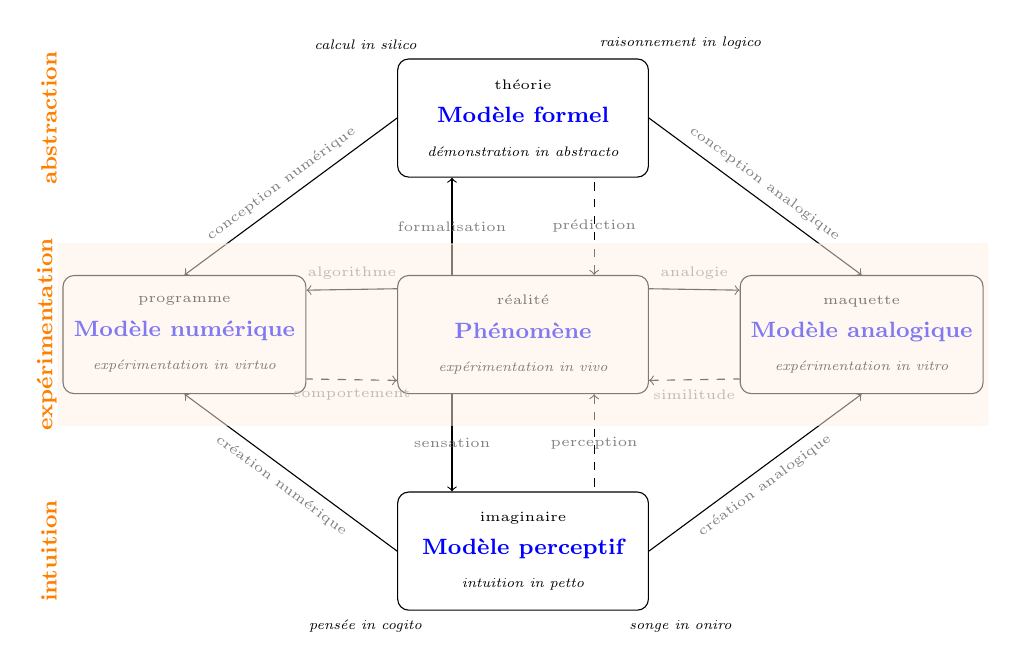
\begin{tikzpicture}
\node[draw,rectangle,rounded corners=4pt,minimum height=1.5cm] (invivo)   at (0,0)  {\begin{minipage}{2.95cm}\begin{center}\mbox{\tiny réalité}\\{\color{blue}\bf\footnotesize Phénomène}\\{\tiny\em expérimentation in vivo}\end{center}\end{minipage}};

\pause

\node[draw,rectangle,rounded corners=4pt,minimum height=1.5cm] (inpetto)   at (0,-2.75)  {\begin{minipage}{2.95cm}\begin{center}\mbox{\tiny imaginaire}\\{\color{blue}\bf\footnotesize Modèle perceptif}\\{\tiny\em intuition in petto}\end{center}\end{minipage}};
\draw[->] (invivo.220) -- (inpetto.140) node[midway] {\color{gray}\tiny sensation};
\draw[<-,dashed] (invivo.320) -- (inpetto.40) node[midway] {\color{gray}\tiny perception};

\node[below] (insilico) at (-2,-3.5) {\tiny\em pensée in cogito};
\node[below] (insilico) at (2,-3.5) {\tiny\em songe in oniro};

\pause

\node[draw,rectangle,rounded corners=4pt,minimum height=1.5cm] (inabstracto)   at (0,2.75)  {\begin{minipage}{2.95cm}\begin{center}\mbox{\tiny théorie}\\{\color{blue}\bf\footnotesize Modèle formel}\\{\tiny\em démonstration in abstracto}\end{center}\end{minipage}};
\draw[->] (invivo.140) -- (inabstracto.220) node[midway] {\color{gray}\tiny formalisation};
\draw[<-,dashed] (invivo.40) -- (inabstracto.320) node[midway] {\color{gray}\tiny prédiction};

\node[above] (insilico) at (-2,3.5) {\tiny\em calcul in silico};
\node[above] (insilico) at (2,3.5) {\tiny\em raisonnement in logico};
\pause

\node[draw,rectangle,rounded corners=4pt,minimum height=1.5cm] (invitro)  at (4.3,0)  {\begin{minipage}{2.85cm}\begin{center}{\tiny maquette}\\{\color{blue}\bf\footnotesize Modèle analogique}\\{\tiny\em expérimentation in vitro}\end{center}\end{minipage}};
\draw[->] (invivo.20) -- (invitro.160) node[midway,above] {\color{gray}\tiny analogie};
\draw[<-,dashed] (invivo.340) -- (invitro.200) node[midway,below] {\color{gray}\tiny similitude};

\pause

\node[draw,rectangle,rounded corners=4pt,minimum height=1.5cm] (invirtuo) at (-4.3,0) {\begin{minipage}{2.85cm}\begin{center}{\tiny programme}\\{\color{blue}\bf\footnotesize Modèle numérique}\\{\tiny\em expérimentation in virtuo}\end{center}\end{minipage}};
\draw[->] (invivo.160) -- (invirtuo.20) node[midway,above] {\color{gray}\tiny algorithme};
\draw[<-,dashed] (invivo.200) -- (invirtuo.340) node[midway,below] {\color{gray}\tiny comportement};

\pause

\draw[->] (inpetto.east) -- (invitro.south) node[below,sloped,midway] {\color{gray}\tiny création analogique};
\draw[->] (inpetto.west) -- (invirtuo.south) node[below,sloped,midway] {\color{gray}\tiny création numérique};

\pause

\draw[->] (inabstracto.east) -- (invitro.north) node[above,sloped,midway] {\color{gray}\tiny conception analogique};
\draw[->] (inabstracto.west) -- (invirtuo.north) node[above,sloped,midway] {\color{gray}\tiny conception numérique};

\pause

\draw[color=orange!10,fill=orange!10,opacity=0.5] (-5.9,-1.15) rectangle (5.9,1.15);
\draw(-5.8,0) node[above,rotate=90] {\color{orange}\footnotesize\bf expérimentation};
\draw(-5.8,2.75) node[above,rotate=90] {\color{orange}\footnotesize\bf abstraction};
\draw(-5.8,-2.75) node[above,rotate=90] {\color{orange}\footnotesize\bf intuition};

\end{tikzpicture}

\end{frame}
\note{}
%------------------------------------------

% rv-3.tex

%------------------------------------------
\begin{frame}<presentation>
\frametitle{L'expérimentation in virtuo}
\framesubtitle{Résumé}
%------------------------------------------
%\begin{columns}[T]
%\column{4cm}
%%\noindent\framebox[4cm]{$\rule{0mm}{6.5cm}$}
%\column{10cm}
\alert{\textbf{Réalité Virtuelle :}} vivre une expérience cognitive et sensorimotrice
dans un univers virtuel peuplé d'entités autonomes.
\vspace*{1mm}

\mbox{}\hfill$\rightarrow$ \alert{\bf vivre une expérience de pensée}\mbox{}
\pause
%\vspace*{0.5cm}

$$\begin{tabular}{cc}
\makebox[4.5cm][c]{\bf Simulation} & \makebox[4.5cm][c]{\bf Jeu de rôle}\\
$\downarrow$ & $\downarrow$ \\
expérimentation in silico & expérimentation in vivo\\
\multicolumn{1}{r}{\pause$\searrow$} & \multicolumn{1}{l}{$\swarrow$}\\
\multicolumn{2}{c}{mettre l'« homme dans la boucle » de simulation}\\
\multicolumn{2}{c}{$\downarrow$}\\
\multicolumn{2}{c}{\alert{\bf expérimentation in virtuo}}
\end{tabular}$$

\pause

\mbox{}\hfill{\footnotesize
\begin{tabular}{l}
\hline
Une autre \begin{minipage}{1cm}\includegraphics[height=1.225cm]{logo-pintofscience}\end{minipage} ? 
\begin{tabular}{l@{$\rightarrow$}l}
oui & \ref{letemps} \\
non & \ref{pasletemps}
\end{tabular}
\end{tabular}}

%\end{columns}
\end{frame}
\note{
Le réalité virtuelle nous permet donc de « vivre des expériences de pensée »

CLIC

et pour vivre de telles expériences de pensée, constitutives de la connaissance elle-même,
elle mixe l'expérimentation in silico des simulations numériques classiques
à l'expérimentation in vivo des jeux de rôle théâtraux

CLIC

afin d'immerger l'homme dans la boucle de simulation pour donner ce que nous appelons
l'expérimentation in virtuo.
Et c'est cette expérimentation in virtuo qui rend possible le vécu d'une expérience 
de pensée et permet une co-construction,
entre l'utilisateur et un système de réalité virtuelle, de nouvelles connaissances.

Alors justement posons-nous la question de la connaissance.
CLIC
}
%------------------------------------------

%------------------------------------------
\begin{frame}<presentation>
\frametitle{Métaconnaissance}
%------------------------------------------
\label{letemps}
%\begin{columns}[T]
%\column{4cm}
%%\noindent\framebox[4cm]{$\rule{0mm}{6.5cm}$}
%\column{10cm}
\vspace*{-2mm}
\begin{description}
\item<2->[SC :] décrire, comprendre la connaissance
\item<3->[IA :] acquérir, représenter, inférer la connaissance
\item<4->[RV :] donner du sens, se construire une connaissance
\end{description}
\vspace*{2mm}

\begin{columns}
\column{6cm}
%\centerline{\includegraphics[width=6cm]{cognition.pdf}}

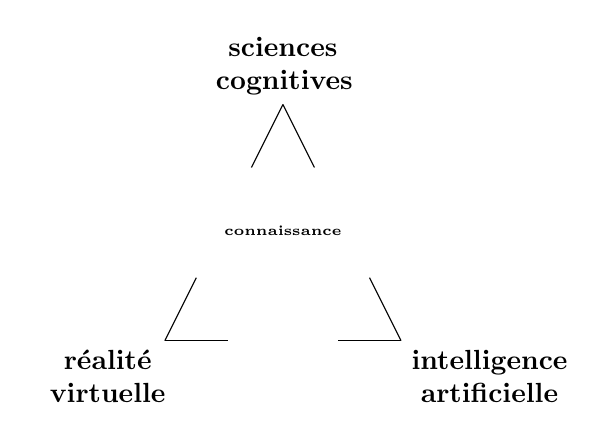
\begin{tikzpicture}
\node (k) at (0,-0.6) {\alert{\bf\tiny connaissance}};

\node[above] (sc) at (0,1) {\begin{minipage}{1.7cm}\begin{center}\bf sciences\\cognitives\end{center}\end{minipage}};

\node[below left] (rv) at (-1.2,-2)  {\begin{minipage}{1.8cm}\begin{center}\bf réalité\\virtuelle\end{center}\end{minipage}};

\node[below right] (ia) at (1.5,-2)  {\begin{minipage}{2cm}\begin{center}\bf intelligence\\artificielle\end{center}\end{minipage}};

\draw(-1.5,-2) -- (-1.1,-1.2);
\draw(-1.5,-2) -- (-0.7,-2);

\draw(1.5,-2) -- (1.1,-1.2);
\draw(1.5,-2) -- (0.7,-2);

\draw(0,1) -- (-0.4,0.2);
\draw(0,1) -- (0.4,0.2);

\end{tikzpicture}

%\pause
\column{4cm}
%Approches :
\begin{itemize}
\item<5-> behaviorisme
\item<6-> computationnalisme
\item<7-> connexionnisme
\item<8-> énactionnisme
\end{itemize}
\end{columns}
%\end{columns}

\end{frame}
\note{
Les sciences cognitives, l'intelligence artificielle et la réalité virtuelle
nous proposent aujourd'hui 3 points de vue sur la connaissance pour éclairer
notre connaissance de la connaissance.

CLIC

Pour simplifier, les sciences cognitives qui ont pour objet d'étude la connaissance 
elle-même, nous aide à décrire et à comprendre la connaissance.

CLIC

De son côté, l'intelligence artificielle se pose la question de l'acquisition 
de la connaissance, de sa représentation informatique afin d'inférer automatiquement 
de nouvelles connaissances.

CLIC

Quant à la réalité virtuelle avec l'expérimentation in virtuo, elle nous permet de donner 
du sens à la connaissance et de se construire une connaissance.

CLIC

Plusieurs courants ont marqué l'histoire des sciences cognitives et de la cognition, 
le processus d'acquisition de la connaissance :
- le behaviorisme tout d'abord où ce processus est vu comme une boîte noire 
	qui agirait à la manière d'une fonction de transfert entre ses entrées et ses sorties,
	entre des stimuli et des réactions, à la manière du chien de Pavlov;

CLIC

- le computationnalisme où on ouvre la boîte noire pour y voir un système de traitement
	de l'information et comparer la cognition à un calcul à la manière d'un ordinateur qui
	exécute des algorithmes;
	
CLIC

- le connexionnisme qui voit la cognition comme un processus émergent de réseaux d'unités simples
	interconnectées, à la manière des réseaux de neurones formels comme ils sont
	aujourd'hui très utilisés en intelligence artificielle dans les algorithmes de deep
	learning (apprentissage profond) par exemple;

CLIC

- et l'énactionnisme qui étend l'approche connexionnisme des réseaux de neurones intracraniens
	en les immergeant dans leur environnement, le processus d'acquisition de la connaissance
	étant alors constitutif du couplage entre l'homme et son environnement.
	
C'est évidemment cette dernière approche que nous retenons pour la réalité virtuelle.

CLIC
}
%------------------------------------------


%------------------------------------------
\begin{frame}<presentation>
\frametitle{Enaction}
%------------------------------------------
%\begin{columns}[T]
%\column{4cm}
%%\noindent\framebox[4cm]{$\rule{0mm}{6.5cm}$}
%\column{10cm}
\begin{block}{Enaction\hfill\tiny Varela F., Invitation aux sciences cognitives, 1996}
histoire du couplage structurel d'une entité autopoiétique avec son environnement,
qui fait émerger un monde
\end{block}
\vspace*{3mm}

\pause
\centerline{\includegraphics[height=3.8cm]{escher-hands.png}
\hspace*{1cm}\includegraphics[height=3.8cm]{escher-gallery.jpg}}

\vspace*{3mm}

\pause
\centerline{\alert{\bf « La marche pour chemin »}}
%\end{columns}

\end{frame}
\note{
L'énaction est un concept introduit à la fin des années 1980 par un biologiste
chilien, Franscesco Varela, qui voyait dans la cognition un processus historique,
celui du couplage structurel qui existe nécessairement entre une entité autonome et 
son environnement. Et de cette dynamique du couplage émerge les connaissances.

CLIC

Pour illustrer cette notion, j'aime bien présenter ces 2 lithographies d'Escher,
un artiste hollandais du 20ème siècle.
La pemière, à gauche, représente 2 mains qui se dessinent mutuellement; l'une n'existe pas 
sans l'autre : d'une certaine manière elles se co-dessinent.
La deuxième, à droite, représente une galerie d'art dans laquelle un usager plonge par la pensée
dans l'un des tableaux dont le bâtiment de droite est la galerie d'art elle-même où il se trouve;
toujours ce couplage entre l'entité et son environnement.

CLIC

Enfin, s'il fallait l'illustrer par une expression, je choisis volontiers
« la marche pour chemin » : c'est en marchant que l'on crée son chemin et une fois créé
il vous aide, vous et d'autres, à aller plus loin lorsque vous repassez par là.
De tout temps, on a adapté notre environnement à nos besoins mais on s'est aussi
adapté à notre environnement.

Mais revenons à la réalité virtuelle :
en quoi ce concepts d'énaction intéresse-t-il la réalité virtuelle ?

CLIC
}
%------------------------------------------


%------------------------------------------
\begin{frame}<presentation>
\frametitle{\mbox{Histoires de couplages structurels}}
%------------------------------------------
%\begin{columns}[T]
%\column{4cm}
%%\noindent\framebox[4cm]{$\rule{0mm}{6.5cm}$}
%\column{10cm}
\begin{description}
\item[Principe de présence :] permettre une activité sensori-motrice dans un monde artificiel\\ {\em $\rightarrow$ « mettre l'homme dans la boucle »}\\
couplage homme $\leftrightarrow$ environnement virtuel
\pause
\vspace*{3mm}

\item[Principe d'autonomie :] permettre une activité «~sensori-motrice » aux entités numériques\\ {\em $\rightarrow$ « autonomiser les entités virtuelles »}\\
couplage entité virtuelle $\leftrightarrow$ entité virtuelle
\pause
\vspace*{3mm}

\item[Principe de substitution :] se mettre à la place d'une entité virtuelle\\
	{\em $\rightarrow$ « passer de la $3^{\grave eme}$ à la $1^{\grave ere}$  personne »}\\
« empathie numérique »

\end{description}
%\end{columns}
\end{frame}
\note{
En fait, la réalité virtuelle est remplie d'histoire de couplages.

Dans ce que j'appelle le 1er principe de la réalité virtuelle : le principe de présence
qui permet une activité sensori-motrice dans un monde artificiel en mettant l'homme dans la boucle,
on instaure un premier couplage entre l'homme, entité autonome,
et l'environnement virtuel.

CLIC

Ce que j'appelle le second principe de la réalité virtuelle : le principe d'autonomie
qui en permettant une activité sensori-motrice aux entités numériques, en les autonomisant
autorise un couplage entre ces entités elles-mêmes.

CLIC

Enfin, le 3ème principe : le principe de substitution qui par empathie numérique permet de se mettre
à la place d'une entité numérique  et de coupler 2 points de vue :
le point de vue à la 3ème personne (celui de l'observateur) et le point de vue à la 1ère personne
(celui de l'acteur).

L'ensemble de ces principes et de leur mise en oeuvre en réalité virtuelle instrumentalise en fait le concepts d'énaction
selon lequel la construction des connaissances et liée à la dynamique des couplages entre une entité 
autonome et son environnement.

CLIC
}
%------------------------------------------

%------------------------------------------
\begin{frame}<presentation>
\frametitle{L'énaction en action}
\framesubtitle{Résumé}
%------------------------------------------
\label{pasletemps}
%\begin{columns}[T]
%\column{4cm}
%	%\noindent\framebox[4cm]{$\rule{0mm}{6.5cm}$}
%\column{10cm}

	\begin{columns}[T]
	\column{8cm}
		\centerline{$\displaystyle\left.\begin{tabular}{l@{\ $\rightarrow$\ }l}
		cri  & langage\\
		oral & écrit  \\
		\hline
		main & outil  
		\end{tabular}\pause
		\right|
		\begin{tabular}{l@{\ $\rightarrow$\ }l}
		réel & virtuel
		\end{tabular}$}
		\vspace*{3mm}
		
		\pause
		\begin{center}
		\alert{\textbf{vivre une expérience de pensée}}\\
		pour co-construire de nouvelles connaissances\\
		et passer des idées reçues, ou conçues, \\
		aux idées vécues
		\end{center}
		\vspace*{2mm}
		
		\pause
		\centerline{\includegraphics[width=6cm]{logo-virtuoscope.jpg}}
	\column{3.5cm}
		%\pause
		
		\mbox{}\hfill\includegraphics[height=6cm]{pinocchio_cerv-blanc.png}
		$\hspace*{-1.mm}\rule{3.75mm}{6cm}$
		
		\mbox{}\hfill\alert{\Huge\sc Merci}
	\end{columns}
%\end{columns}

\end{frame}
\note{
Pour conclure cette petite épistémologie de la réalité virtuelle, rappelons
que l'homme de tout temps a créé des artefacts qui fondamentalement l'ont aidé 
à construire son humanité.


}
%------------------------------------------


%------------------------------------------
\begin{frame}
%------------------------------------------
\vspace*{3mm}

\includegraphics[height=1.225cm]{logo-cerv}\hfill
\includegraphics[height=1.225cm]{logo-pintofscience}\includegraphics[height=1.225cm]{logo-pintofscience}\includegraphics[height=1.225cm]{logo-pintofscience}

\setbeamercolor{block body}{fg=white,bg=orange}
\begin{block}{}
\centerline{\huge\bf
\begin{tabular}{c}
\mbox{}\\
\cellcolor{orange}\color{white}Réalité virtuelle\\
\mbox{}
\end{tabular}
}
\end{block}
\setbeamercolor{block body}{fg=black,bg=white}
\null\vfill

\centerline{\LARGE Jacques Tisseau}
\null\vfill

\noindent
%\mbox{}\hfill
\begin{minipage}{1.5cm}
\includegraphics[height=1.3cm]{logo-cnrs}
\end{minipage}
\hspace{-4mm}
\begin{minipage}{3cm}
\includegraphics[height=1.3cm]{logo-labsticc}
\end{minipage}
\hfill
\begin{minipage}{2.75cm}
\begin{center}
%\includegraphics[height=1.75cm]{logo-pintofscience}\\
%16/05/2018
\end{center}
\end{minipage}
\hfill
\begin{minipage}{2.75cm}
\includegraphics[height=1.75cm]{logo-enib}
\end{minipage}
%\hfill
\mbox{}

\end{frame}
\note{}
%------------------------------------------


%-------------------------------------------------------------------------
\end{document}
%-------------------------------------------------------------------------




